\documentclass[tikz,border=6pt]{standalone}
\usepackage{amsmath}
\usepackage{newtxtext,newtxmath}
\usetikzlibrary{arrows.meta,calc,positioning,shapes.geometric}

\begin{document}
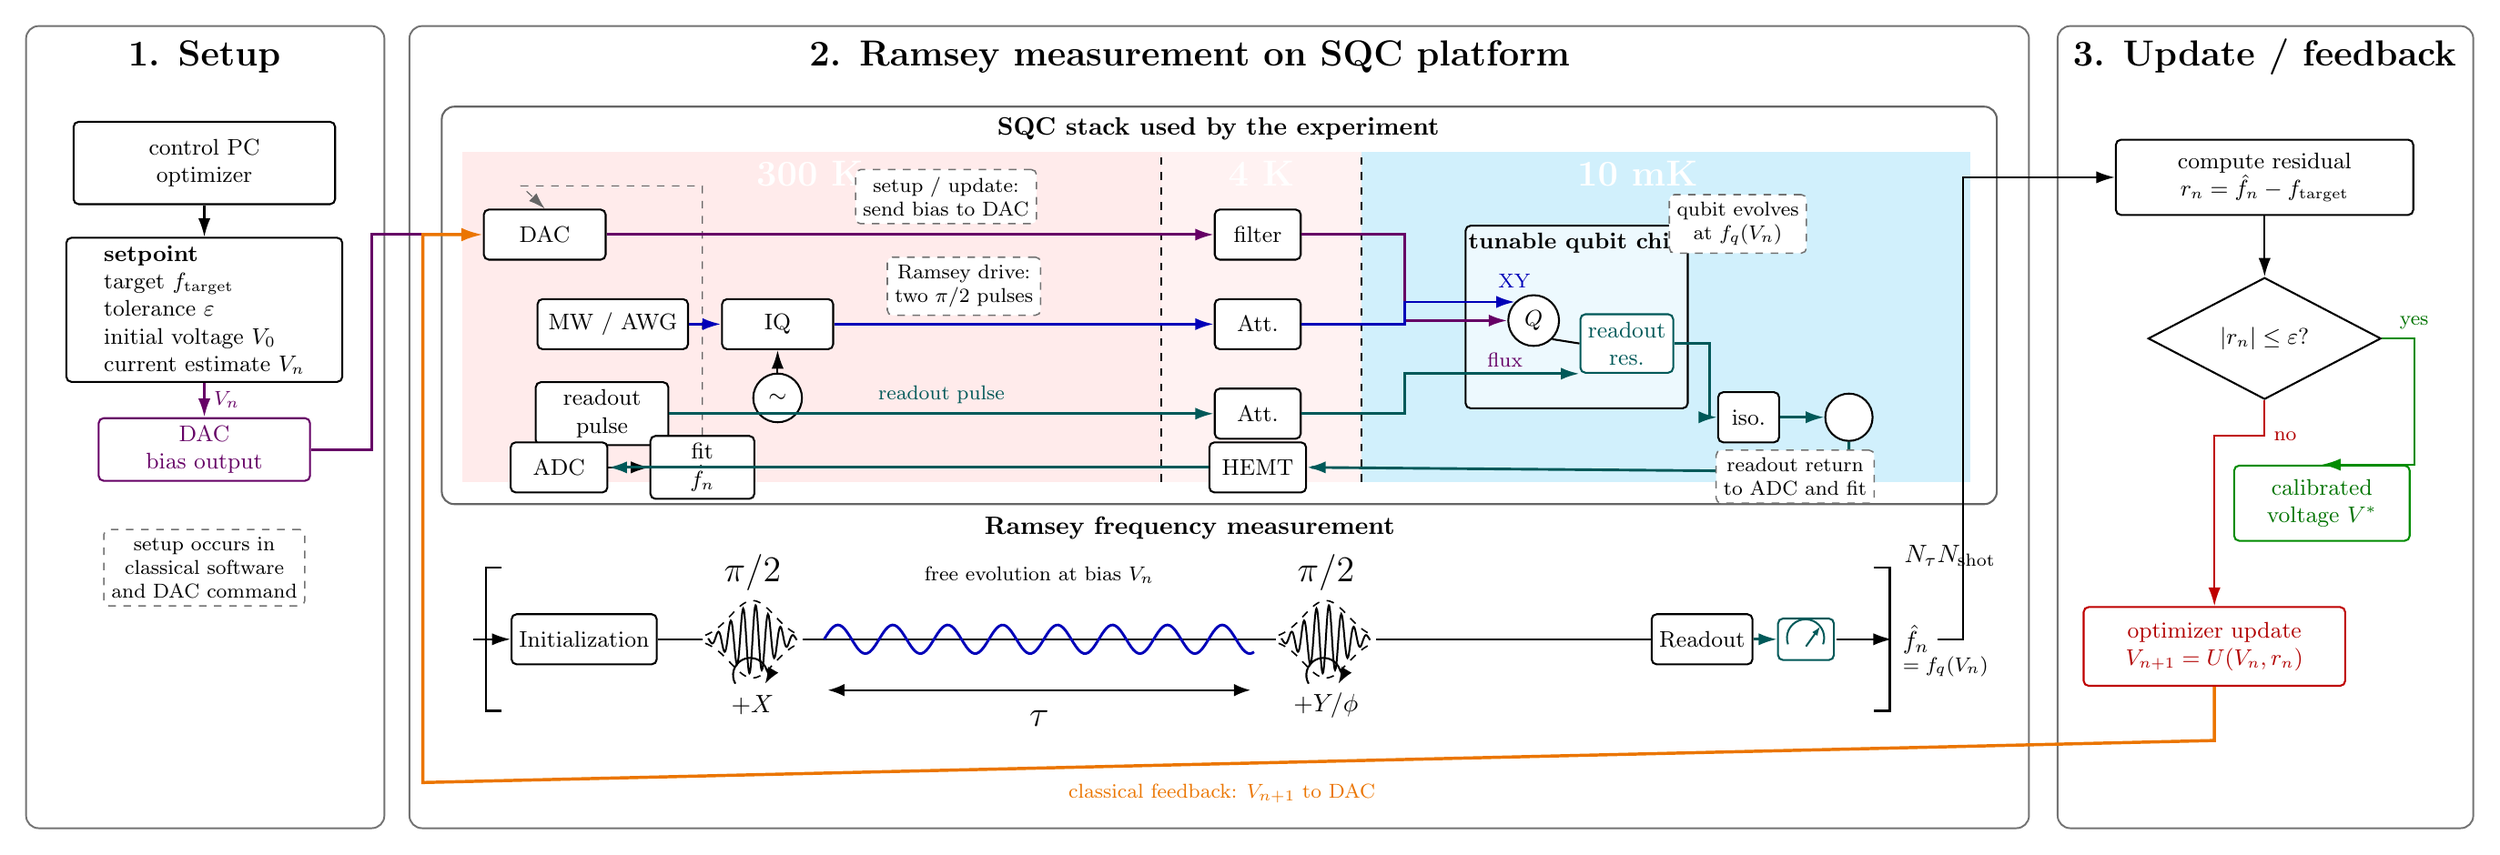
\begin{tikzpicture}[
  x=1cm,
  y=1cm,
  >=Latex,
  font=\small,
  line/.style={draw=black,line width=0.75pt},
  frame/.style={draw=black!60,line width=0.75pt,rounded corners=5pt},
  panel/.style={draw=black!55,line width=0.7pt,rounded corners=5pt,fill=white},
  box/.style={line,rounded corners=2pt,fill=white,align=center,minimum height=0.70cm,inner sep=3pt},
  chipbox/.style={line,rounded corners=2pt,fill=white,align=center,inner sep=3pt},
  xy/.style={draw=blue!72!black,line width=1.05pt},
  flux/.style={draw=violet!80!black,line width=1.05pt},
  ro/.style={draw=teal!70!black,line width=1.05pt},
  feed/.style={draw=orange!92!black,line width=1.25pt},
  xyarr/.style={xy,-{Latex[length=2.6mm,width=1.7mm]}},
  fluxarr/.style={flux,-{Latex[length=2.6mm,width=1.7mm]}},
  roarr/.style={ro,-{Latex[length=2.6mm,width=1.7mm]}},
  feedarr/.style={feed,-{Latex[length=3.0mm,width=1.9mm]}},
  blkarr/.style={line,-{Latex[length=2.6mm,width=1.7mm]}},
  callout/.style={draw=black!55,dashed,line width=0.55pt,rounded corners=2pt,fill=white,align=center,font=\footnotesize,inner sep=3pt},
  pulse/.style={draw=black,line width=0.72pt},
  env/.style={draw=black,dashed,line width=0.58pt},
  temp/.style={font=\bfseries\Large,text=white,align=center},
  labxy/.style={font=\footnotesize,text=blue!72!black,align=center},
  labflux/.style={font=\footnotesize,text=violet!80!black,align=center},
  labro/.style={font=\footnotesize,text=teal!70!black,align=center},
  labfeed/.style={font=\footnotesize,text=orange!92!black,align=center}
]

% ---------------------------------------------------------------------------
% Main panels
\node[panel,minimum width=5.0cm,minimum height=11.2cm,anchor=south west] (setupPanel) at (0,0) {};
\node[panel,minimum width=22.6cm,minimum height=11.2cm,anchor=south west] (measurePanel) at (5.35,0) {};
\node[panel,minimum width=5.8cm,minimum height=11.2cm,anchor=south west] (updatePanel) at (28.35,0) {};

\node[font=\bfseries\Large] at (2.50,10.78) {1. Setup};
\node[font=\bfseries\Large] at (16.25,10.78) {2. Ramsey measurement on SQC platform};
\node[font=\bfseries\Large] at (31.25,10.78) {3. Update / feedback};

% ---------------------------------------------------------------------------
% Setup panel
\node[box,minimum width=3.65cm,minimum height=1.15cm] (setCPU) at (2.50,9.30)
  {control PC\\optimizer};
\node[box,minimum width=3.85cm,minimum height=1.75cm,align=left] (setList) at (2.50,7.25)
  {\textbf{setpoint}\\
   target $f_{\mathrm{target}}$\\
   tolerance $\varepsilon$\\
   initial voltage $V_0$\\
   current estimate $V_n$};
\node[box,minimum width=2.95cm,draw=violet!80!black,text=violet!80!black] (setDAC) at (2.50,5.30)
  {DAC\\bias output};
\draw[blkarr] (setCPU.south) -- (setList.north);
\draw[fluxarr] (setList.south) -- node[right,font=\footnotesize,text=violet!80!black] {$V_n$} (setDAC.north);
\node[callout] at (2.50,3.65) {setup occurs in\\classical software\\and DAC command};

% Arrow from setup into measurement platform.
\draw[fluxarr] (setDAC.east) -- ++(0.85,0) |- (6.80,8.30);

% ---------------------------------------------------------------------------
% Simplified SQC stack inside measurement panel
\node[frame,minimum width=21.7cm,minimum height=5.55cm,anchor=north west] (stackFrame) at (5.80,10.10) {};
\node[font=\bfseries] at (16.65,9.78) {SQC stack used by the experiment};

% Temperature zones within stack
\fill[pink!32] (6.10,4.85) rectangle (15.85,9.45);
\fill[pink!20] (15.85,4.85) rectangle (18.65,9.45);
\fill[cyan!18] (18.65,4.85) rectangle (27.15,9.45);
\draw[black,dashed,line width=0.75pt] (15.85,4.85) -- (15.85,9.45);
\draw[black,dashed,line width=0.75pt] (18.65,4.85) -- (18.65,9.45);
\node[temp] at (10.95,9.15) {300 K};
\node[temp] at (17.25,9.15) {4 K};
\node[temp] at (22.50,9.15) {10 mK};

% 300 K blocks
\node[box,minimum width=1.70cm] (dac) at (7.25,8.30) {DAC};
\node[box,minimum width=2.10cm] (mw) at (8.20,7.05) {MW / AWG};
\node[box,minimum width=1.55cm] (iq) at (10.50,7.05) {IQ};
\node[circle,line,minimum size=0.68cm,fill=white] (lo) at (10.50,6.02) {$\sim$};
\node[box,minimum width=1.85cm] (roPulse) at (8.05,5.80) {readout\\pulse};
\node[box,minimum width=1.35cm] (adc) at (7.45,5.05) {ADC};
\node[box,minimum width=1.45cm] (fit) at (9.45,5.05) {fit\\$\hat f_n$};

\draw[blkarr] (lo.north) -- (iq.south);
\draw[blkarr] (adc.east) -- (fit.west);
\draw[black!60,dashed,-{Latex[length=2.3mm,width=1.5mm]}] (fit.north) |- (6.92,8.98) -- (dac.north);

% 4 K minimal chain
\node[box,minimum width=1.20cm] (fluxFilter) at (17.20,8.30) {filter};
\node[box,minimum width=1.20cm] (driveAtt) at (17.20,7.05) {Att.};
\node[box,minimum width=1.20cm] (roAtt) at (17.20,5.80) {Att.};
\node[box,minimum width=1.35cm] (hemt) at (17.20,5.05) {HEMT};

% 10 mK chip
\node[chipbox,minimum width=3.10cm,minimum height=2.55cm,fill=cyan!7] (chip) at (21.65,7.15) {};
\node[font=\bfseries\small] at (21.65,8.18) {tunable qubit chip};
\node[circle,line,minimum size=0.70cm,fill=white] (qubit) at (21.05,7.10) {$Q$};
\node[chipbox,minimum width=1.15cm,draw=teal!70!black,text=teal!70!black] (res) at (22.35,6.78) {readout\\res.};
\draw[line] (qubit.south east) -- (res.west);
\node[labxy] at (20.78,7.65) {XY};
\node[labflux] at (20.65,6.55) {flux};
\node[box,minimum width=0.85cm] (iso) at (24.05,5.75) {iso.};
\node[circle,line,minimum size=0.66cm,fill=white] (circ) at (25.45,5.75) {$\circlearrowright$};

% Relevant paths
\draw[fluxarr] (dac.east) -- node[above,font=\footnotesize,text=violet!80!black] {$V_n$ or $V_{n+1}$} (fluxFilter.west);
\draw[fluxarr] (fluxFilter.east) -- ++(0.45,0) -- (19.25,8.30) |- (qubit.west);
\draw[xyarr] (mw.east) -- (iq.west);
\draw[xyarr] (iq.east) -- (driveAtt.west);
\draw[xyarr] (driveAtt.east) -- ++(0.52,0) -- (19.25,7.05) |- (qubit.north west);
\draw[roarr] (roPulse.east) -- node[above,font=\footnotesize,text=teal!70!black] {readout pulse} (roAtt.west);
\draw[roarr] (roAtt.east) -- ++(0.55,0) -- (19.25,5.80) |- (res.south west);
\draw[roarr] (res.east) -- ++(0.50,0) |- (iso.west);
\draw[roarr] (iso.east) -- (circ.west);
\draw[roarr] (circ.south) -- ++(0,-0.42) -- (17.95,5.05) -- (hemt.east);
\draw[roarr] (hemt.west) -- (adc.east);

% Compact operation labels in stack.
\node[callout] at (12.85,8.83) {setup / update:\\send bias to DAC};
\node[callout] at (13.10,7.58) {Ramsey drive:\\two $\pi/2$ pulses};
\node[callout] at (23.90,8.45) {qubit evolves\\at $f_q(V_n)$};
\node[callout] at (24.70,4.92) {readout return\\to ADC and fit};

% ---------------------------------------------------------------------------
% Ramsey sequence below stack
\node[font=\bfseries] at (16.25,4.20) {Ramsey frequency measurement};
\coordinate (seqL) at (6.65,2.65);
\coordinate (seqR) at (25.80,2.65);
\draw[line width=1.0pt] ($(seqL)+(0,1.00)$) -- ++(-0.22,0) -- ++(0,-2.00) -- ++(0.22,0);
\draw[line width=1.0pt] ($(seqR)+(0,1.00)$) -- ++(0.22,0) -- ++(0,-2.00) -- ++(-0.22,0);
\node[anchor=south west,font=\normalsize] at ($(seqR)+(0.30,0.90)$) {$N_\tau N_{\mathrm{shot}}$};

\node[box,minimum width=1.55cm] (init) at (7.80,2.65) {Initialization};
\node[box,minimum width=1.25cm] (rout) at (23.40,2.65) {Readout};
\draw[blkarr] (6.25,2.65) -- (init.west);
\draw[line] (init.east) -- (9.45,2.65);
\draw[line] (10.85,2.65) -- (17.45,2.65);
\draw[line] (18.85,2.65) -- (rout.west);
\draw[roarr] (rout.east) -- (24.45,2.65);

% Ramsey pulses
\begin{scope}[shift={(10.15,2.65)}]
  \node[font=\Large] at (0,0.93) {$\pi/2$};
  \draw[pulse,domain=-0.62:0.62,samples=130,smooth]
    plot (\x,{0.48*exp(-6.6*\x*\x)*sin(deg(36*\x))});
  \draw[env,domain=-0.66:0.66,samples=80,smooth]
    plot (\x,{0.54*exp(-5.2*\x*\x)});
  \draw[env,domain=-0.66:0.66,samples=80,smooth]
    plot (\x,{-0.54*exp(-5.2*\x*\x)});
  \draw[->,line width=0.75pt] (-0.24,-0.62) arc[start angle=210,end angle=-30,radius=0.24];
  \node[font=\normalsize] at (0,-0.92) {$+X$};
\end{scope}

\begin{scope}[shift={(18.15,2.65)}]
  \node[font=\Large] at (0,0.93) {$\pi/2$};
  \draw[pulse,domain=-0.62:0.62,samples=130,smooth]
    plot (\x,{0.48*exp(-6.6*\x*\x)*sin(deg(36*\x))});
  \draw[env,domain=-0.66:0.66,samples=80,smooth]
    plot (\x,{0.54*exp(-5.2*\x*\x)});
  \draw[env,domain=-0.66:0.66,samples=80,smooth]
    plot (\x,{-0.54*exp(-5.2*\x*\x)});
  \draw[->,line width=0.75pt] (-0.24,-0.62) arc[start angle=210,end angle=-30,radius=0.24];
  \node[font=\normalsize] at (0,-0.92) {$+Y/\phi$};
\end{scope}

\draw[xy,domain=11.15:17.15,samples=190,smooth]
  plot (\x,{2.65 + 0.20*sin(deg(8.2*(\x-11.15)))});
\draw[Latex-Latex,line width=0.80pt] (11.20,1.94) -- (17.10,1.94);
\node[font=\Large] at (14.15,1.55) {$\tau$};
\node[font=\footnotesize,align=center] at (14.15,3.55) {free evolution at bias $V_n$};

% Meter and extracted frequency
\node[box,minimum width=0.78cm,minimum height=0.58cm,draw=teal!70!black] (meter) at (24.85,2.65) {};
\draw[ro,line width=0.72pt] (24.60,2.58) arc[start angle=200,end angle=-20,radius=0.26];
\draw[ro,-{Latex[length=1.3mm,width=0.9mm]},line width=0.72pt] (24.85,2.55) -- (25.05,2.83);
\draw[blkarr] (25.28,2.65) -- (26.05,2.65);
\node[anchor=west,font=\normalsize] (fhat) at (26.08,2.65) {$\hat f_n$};
\node[anchor=west,font=\footnotesize] at (26.08,2.27) {$=f_q(V_n)$};

% ---------------------------------------------------------------------------
% Update panel
\node[box,minimum width=4.15cm,minimum height=1.05cm] (resid) at (31.25,9.10)
  {compute residual\\$r_n=\hat f_n-f_{\mathrm{target}}$};
\node[diamond,line,aspect=1.85,inner sep=1.5pt,minimum width=3.25cm,minimum height=1.70cm,align=center] (decide) at (31.25,6.85)
  {$|r_n|\leq\varepsilon$?};
\node[box,minimum width=2.45cm,minimum height=1.05cm,draw=green!55!black,text=green!45!black] (done) at (32.05,4.55)
  {calibrated\\voltage $V^\ast$};
\node[box,minimum width=3.65cm,minimum height=1.10cm,draw=red!75!black,text=red!70!black] (upd) at (30.55,2.55)
  {optimizer update\\$V_{n+1}=U(V_n,r_n)$};
\draw[blkarr] (resid.south) -- (decide.north);
\draw[line,draw=green!55!black,-{Latex[length=2.6mm,width=1.7mm]}]
  (decide.east) -- ++(0.45,0) node[above,font=\footnotesize,text=green!45!black] {yes} |- (done.north);
\draw[line,draw=red!75!black,-{Latex[length=2.6mm,width=1.7mm]}]
  (decide.south) -- ++(0,-0.50) node[right,font=\footnotesize,text=red!70!black] {no} -| (upd.north);
\draw[blkarr] (fhat.east) -- ++(0.35,0) |- (resid.west);

% Feedback loop returns to DAC, not directly to chip.
\draw[feedarr] (upd.south) -- ++(0,-0.75) -- (5.55,0.65) -- (5.55,8.30) -- (dac.west);
\node[labfeed,fill=white,inner sep=1pt] at (16.70,0.50) {classical feedback: $V_{n+1}$ to DAC};

\end{tikzpicture}
\end{document}
